\documentclass[10pt]{beamer}
%\documentclass[handout,10pt]{beamer}
%\mode<presentation>
%{
%  \usetheme{Berkeley}
%  \usecolortheme{seahorse}
%  \usefonttheme{default}
%  \setbeamertemplate{navigation symbols}{}
%  \setbeamertemplate{caption}[numbered]
%}

\usetheme{metropolis}

\usepackage[english]{babel}
\usepackage[utf8x]{inputenc}
\usepackage{caption}
\usepackage{multirow}
\usepackage{mathrsfs}
\usepackage{graphicx}
\usepackage{amsmath}
\usepackage{graphicx}
\usepackage[compatibility=false]{caption}
\usepackage{subcaption}
\usepackage[normalem]{ulem}
\DeclareMathOperator{\tr}{tr}
\usepackage{textpos}
\usepackage{animate}
\DeclareMathOperator{\sech}{sech}
\DeclareMathOperator{\cosech}{cosech}
\DeclareMathOperator{\cosec}{cosec}

\title[FMSP Further Mathematics]{Hyperbolics}
%\titlegraphic{\includegraphics[height=1.57cm]{logo.jpg}}
\author[Scott Morgan]{\textbf{Scott Morgan}}
\institute{\textit{Further Mathematics Support Programme - WJEC A-Level Further Mathematics} \\
\textit{31st March 2018}
\\ \\ \\
\textit{scott3142.com | @Scott3142}}
\date

\begin{document}

\begin{frame}
  \maketitle
\end{frame}

\begin{frame}{Topics}
  \begin{itemize}
	  \item Hyperbolic Identities
 	  \item Calculus with Hyperbolics - Differentiation \& Integration
	  \item Inverse Hyperbolic Functions
  \end{itemize}
\end{frame}

\begin{frame}{Topics}
  \begin{itemize}
	  \item Hyperbolic Identities
  \end{itemize}
\end{frame}

\begin{frame}{Hyperbolic Functions}

	\begin{align*}
		\sinh(x) \only<2->{&= \frac{e^x - e^{-x}}{2}} \\
		\cosh(x) \only<2->{&= \frac{e^x + e^{-x}}{2}}
	\end{align*}

\end{frame}

\begin{frame}{Hyperbolic Functions}

	\begin{equation*}
		y = \sinh(x)
	\end{equation*}

	\begin{figure}
		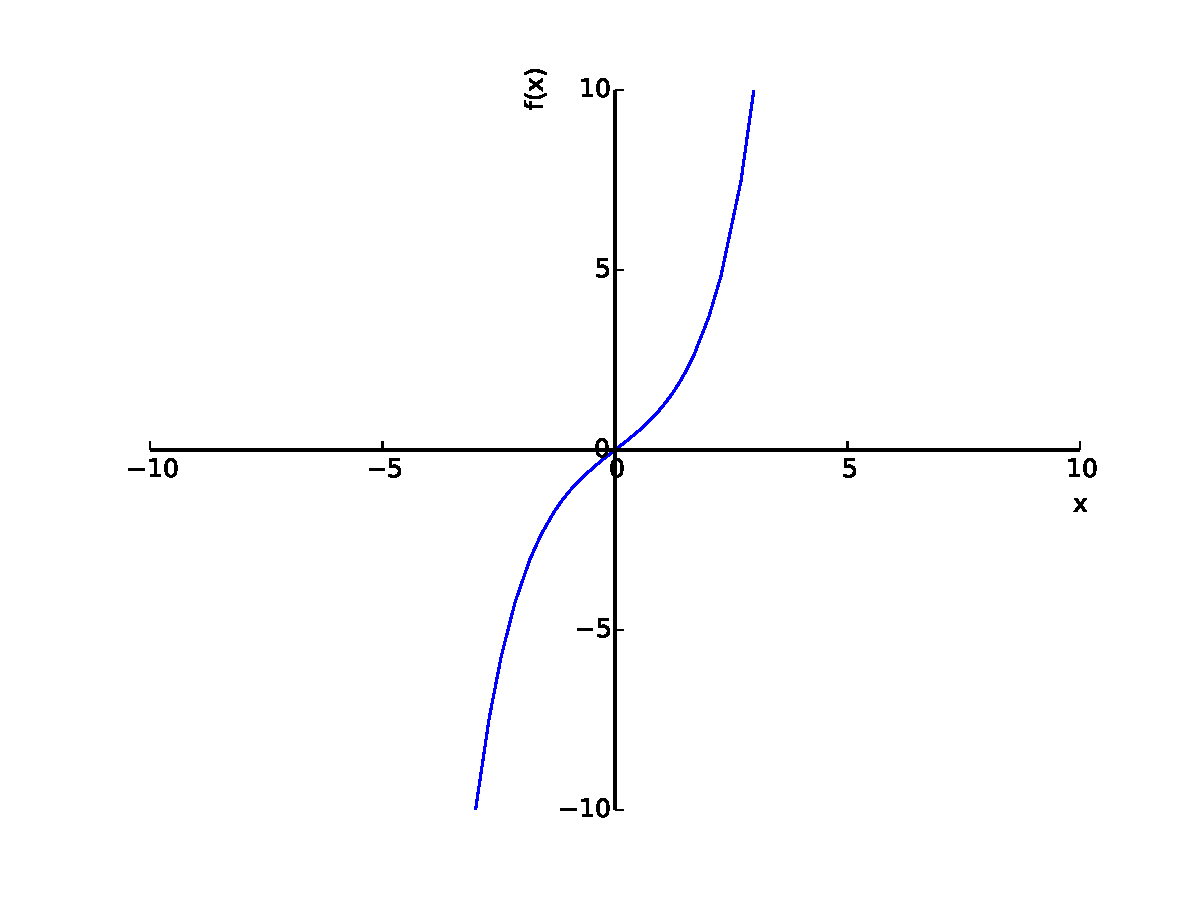
\includegraphics[width=0.8\textwidth]{beamer-pics/hyperbolics-1.pdf}
	\end{figure}

\end{frame}

\begin{frame}{Hyperbolic Functions}

	\begin{equation*}
		y = \cosh(x)
	\end{equation*}

	\begin{figure}
		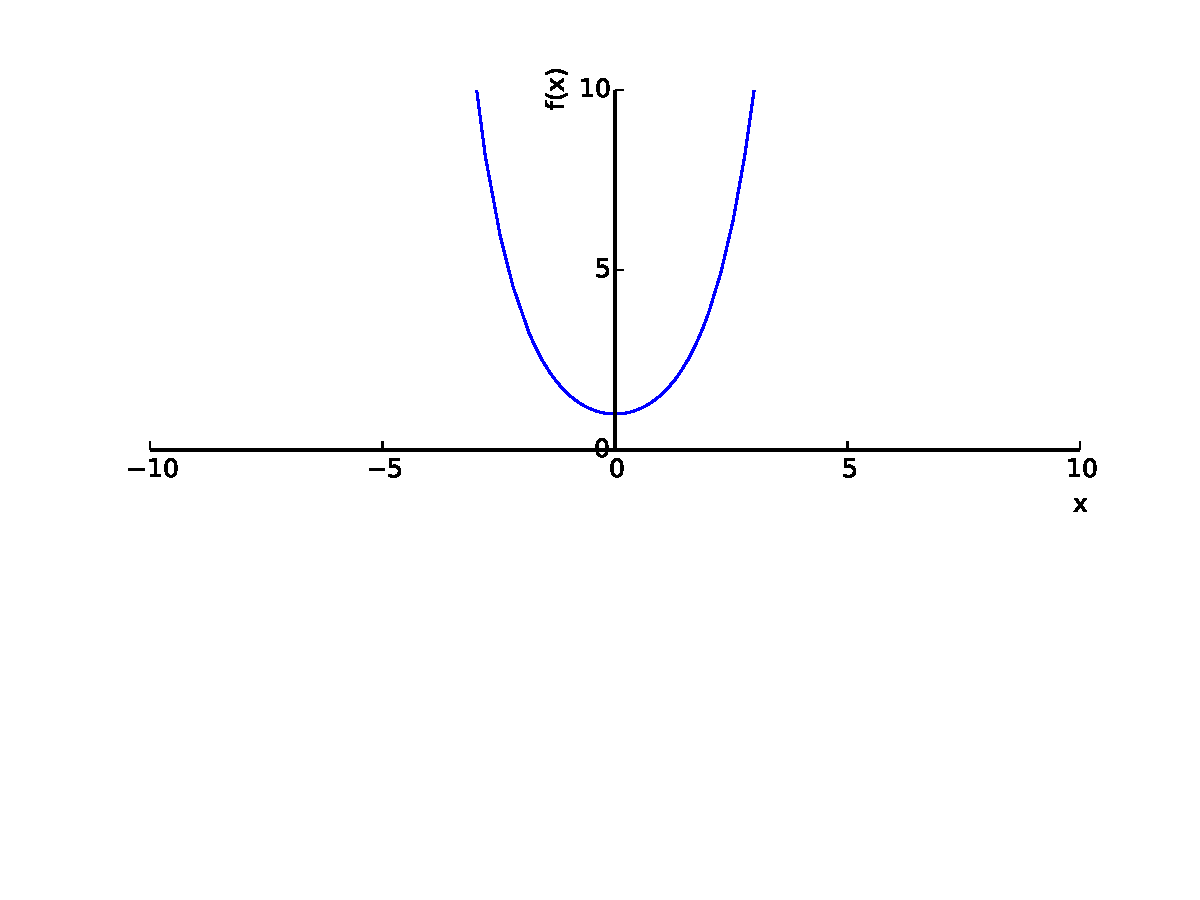
\includegraphics[width=0.9\textwidth]{beamer-pics/hyperbolics-2.pdf}
	\end{figure}

\end{frame}

\begin{frame}{Hyperbolic Functions}

	\begin{equation*}
		y = \tanh(x)
	\end{equation*}

	\begin{figure}
		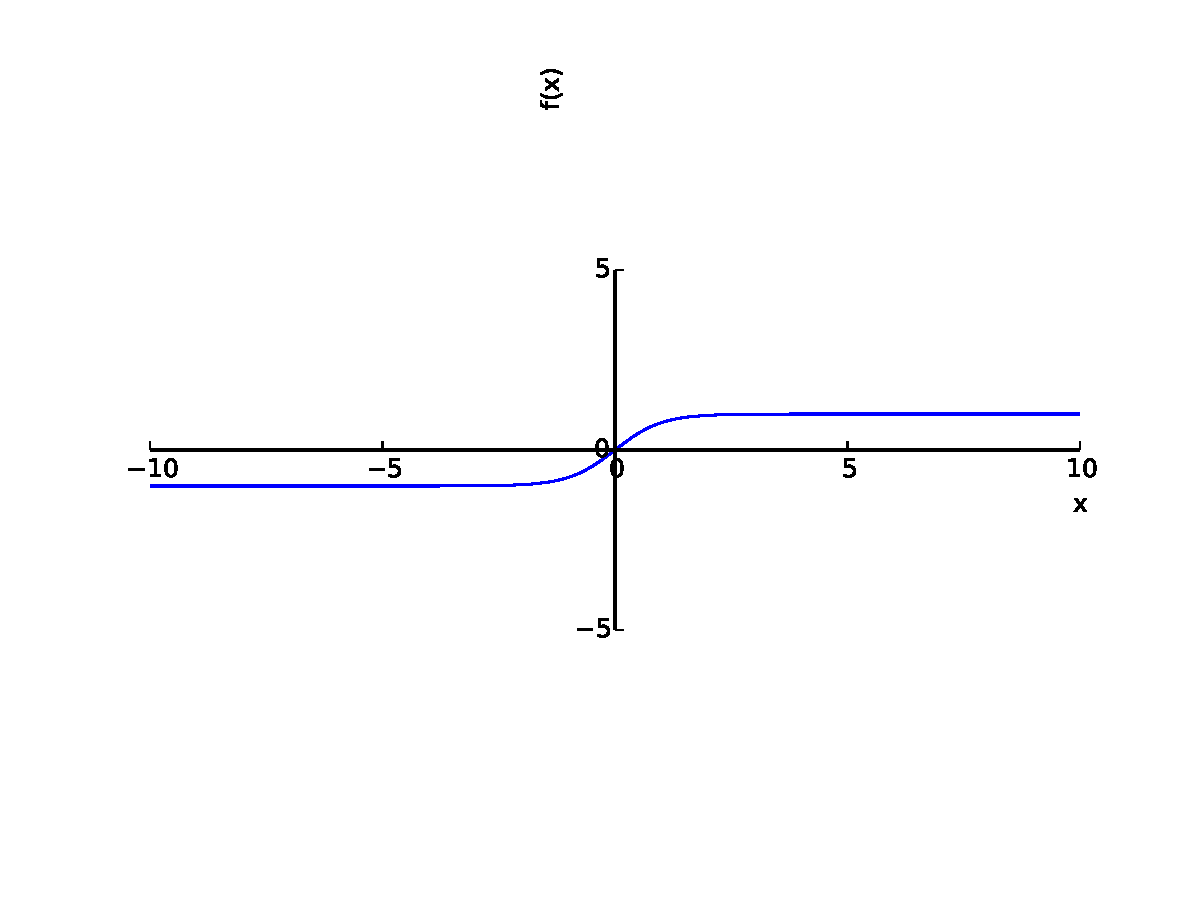
\includegraphics[width=0.9\textwidth]{beamer-pics/hyperbolics-3.pdf}
	\end{figure}

\end{frame}

\begin{frame}{Hyperbolic Functions}

	\begin{align*}
		\tanh(x) &= \frac{\sinh(x)}{\cosh(x)} \only<2-> {= \frac{e^x - e^{-x}}{e^x + e^{-x}}} \\
		\cosech(x) &= \frac{1}{\sinh(x)} \only<2-> {= \frac{2}{e^x - e^{-x}}} \\
		\sech(x) &= \frac{1}{\cosh(x)} \only<2-> {= \frac{2}{e^x + e^{-x}}} \\
		\coth(x) &= \frac{\cosh(x)}{\sinh(x)} \only<2-> {= \frac{e^x + e^{-x}}{e^x - e^{-x}}}
	\end{align*}

\end{frame}

\begin{frame}{Hyperbolic Functions}

	\textbf{Examples:}
	
	Prove the following identities, using the exponential definitions of the hyperbolic functions.
	
	\begin{itemize}
		\item $\cosh^2(x) - \sinh^2(x) = 1$
		\item $\cosh (2x) = 1 + 2\sinh^2(x)$
		\item $\cosh(x+y) = \cosh(x)\cosh(y) + \sinh(x)\sinh(y)$
	\end{itemize}

\end{frame}

\begin{frame}{Trigonometric vs Hyperbolic Identities}
	\begin{center}
	    \begin{tabular}{| l | l |}
	    \hline
	    Trigonometric Identity & Hyperbolic Identity \\ 
	    \hline
	    & \\ $\cos^2(x) + \sin^2(x) = 1$ & $\cosh^2(x) - \sinh^2(x) = 1$ \\ & \\
	    \hline
	    & \\ $1 + \tan^2(x) = \sec^2(x)$ & $1 - \tanh^2(x) = \sech^2(x)$ \\ & \\
	    \hline 
	    & \\ $\cot^2(x) + 1 = \cosec^2(x)$ & $\coth^2(x) - 1 = \cosech^2(x)$ \\ & \\
	    \hline
	    \end{tabular}
	\end{center}
\end{frame}

\begin{frame}{Trigonometric vs Hyperbolic Identities}
	\begin{center}
	    \begin{tabular}{| l | l |}
	    \hline
	    Trigonometric Identity & Hyperbolic Identity \\ 
	    \hline
	    & \\ $\sin(2x) = 2\sin(x)\cos(x)$ & $\sinh(2x) = 2\sinh(x)\cosh(x)$ \\ & \\
	    \hline
	    & \\ $\cos(2x) = \cos^2(x) - \sin^2(x)$ & $\cos(2x) = \cos^2(x) + \sin^2(x)$ \\ & \\
	    \hline 
	    & \\ $\cos (2x) = 2\cos^2(x) - 1$ & $\cosh (2x) = 2\cosh^2(x) - 1$ \\ & \\
	    \hline 
		& \\ $\cos (2x) = 1 - 2\sin^2(x)$ & $\cosh (2x) = 1 + 2\sinh^2(x)$ \\ & \\
		\hline
		& \\ $\tan(2x) = \frac{2\tan(x)}{1-\tan^2(x)}$ & $\tanh(2x) = \frac{2\tanh(x)}{1+\tanh^2(x)}$ \\ & \\
	    \hline
	    \end{tabular}
	\end{center}
\end{frame}

\begin{frame}{Trigonometric vs Hyperbolic Identities}
	\begin{center}
		\scriptsize
	    \begin{tabular}{| l | l |}
	    \hline
	    Trigonometric Identity & Hyperbolic Identity \\ 
	    \hline
	    & \\ $\sin (x + y) = \sin(x)\cos(y) + \cos(x)\sin(y)$ & $\sinh (x + y) = \sinh(x)\cosh(y) + \cosh(x)\sinh(y)$ \\ & \\
	    \hline 
	    & \\ $\sin (x - y) = \sin(x)\cos(y) - \cos(x)\sin(y)$ & $\sinh (x - y) = \sinh(x)\cosh(y) - \cosh(x)\sinh(y)$ \\ & \\
	    \hline 
		& \\ $\cos (x + y) = \cos(x)\cos(y) - \sin(x)\sin(y)$ & $\cosh (x + y) = \cosh(x)\cosh(y) + \sinh(x)\sinh(y)$ \\ & \\
		\hline 
		& \\ $\cos (x - y) = \cos(x)\cos(y) + \sin(x)\sin(y)$ & $\cosh (x - y) = \cosh(x)\cosh(y) - \sinh(x)\sinh(y)$ \\ & \\
	    \hline
	    \end{tabular}
	\end{center}
\end{frame}

\begin{frame}{Equations with Hyperbolic Functions}

	\textbf{Examples:}
	
	Solve the following equations:
	
	\begin{itemize}
		\item $3\sinh(x) - \cosh(x) = 1$
		\item $\tanh(x) + 4\sech(x) = 4$
		\item $12\cosh^2(x) + 7\sinh(x) = 24$
	\end{itemize}

\end{frame}

\begin{frame}{Topics}
  \begin{itemize}
 	  \item Calculus with Hyperbolics - Differentiation \& Integration
  \end{itemize}
\end{frame}

\begin{frame}{Calculus with Hyperbolic Functions - Differentiation}

	\begin{align*}
		\frac{d (\sinh(x))}{dx} \only<2->{&= \frac{d}{dx}\left(\frac{e^x - e^{-x}}{2}\right) = \frac{e^x + e^{-x}}{2} = \cosh(x)} \\
		\frac{d (\cosh(x))}{dx} \only<3->{&= \frac{d}{dx}\left(\frac{e^x + e^{-x}}{2}\right) = \frac{e^x - e^{-x}}{2} = \sinh(x)} 
	\end{align*}

\end{frame}

\begin{frame}{Calculus with Hyperbolic Functions - Differentiation}

	\textbf{Examples:}
	
	Find the derivatives of the following:
	
	\begin{itemize}
		\item $\tanh(x)$
		\item $\cosech(x)$
		\item $\sech(x)$
		\item $\coth(x)$		
	\end{itemize}

\end{frame}

\begin{frame}{Calculus with Hyperbolic Functions - Differentiation}

	\textbf{Examples:}
	
	Find the derivatives of the following:
	
	\begin{itemize}
		\item $\tanh(2x)$
		\item $\sech^2(x)$
		\item $\sinh(4x)$
		\item $\cosh^3(x)$		
		\item $x\sinh(x)$
		\item $e^x\sinh(x)$		
		\item $\sqrt{\cosh(5x)}$		
		\item $e^{\cosh(x)}$		
		\item $\ln(\sinh(x))$
	\end{itemize}

\end{frame}

\begin{frame}{Calculus with Hyperbolic Functions - Integration}

	\begin{align*}
		\int\sinh(x)dx \only<2->{&= \cosh(x) + c} \\
		\int\cosh(x)dx \only<3->{&= \sinh(x) + c} 
	\end{align*}

\end{frame}

\begin{frame}{Calculus with Hyperbolic Functions - Integration}

	\textbf{Examples:}
	
	Find the following:
	
	\begin{itemize}
		\item $\int x\sinh(2x)dx$
		\item $\int \sinh^2(x)dx$
		\item $\int \cosh^2(x)dx$
		\item $\int \sinh(3x)dx$
		\item $\int \cosh(5x)dx$
		\item $\int 3x\cosh(4x)dx$
		\item $\int \sinh(x)\cosh(x)dx$
	\end{itemize}

\end{frame}

\begin{frame}{Topics}
  \begin{itemize}
	  \item Inverse Hyperbolic Functions
  \end{itemize}
\end{frame}

\begin{frame}{Inverse Hyperbolic Functions}

	\textbf{Example:}
	
	Using the exponential definition for $\sinh(x)$, show that
	
	\begin{align*}
		\sinh^{-1}(x) &= \ln\left(x + \sqrt{x^2+1}\right) \\
		\cosh^{-1}(x) &= \ln\left(x + \sqrt{x^2-1}\right) \\
		\tanh^{-1}(x) &= \frac12\ln\left(\frac{1-x}{1+x}\right)
	\end{align*}

\end{frame}

\begin{frame}{Inverse Hyperbolic Functions}

	\begin{equation*}
		y = \sinh^{-1}(x)
	\end{equation*}

	\begin{figure}
		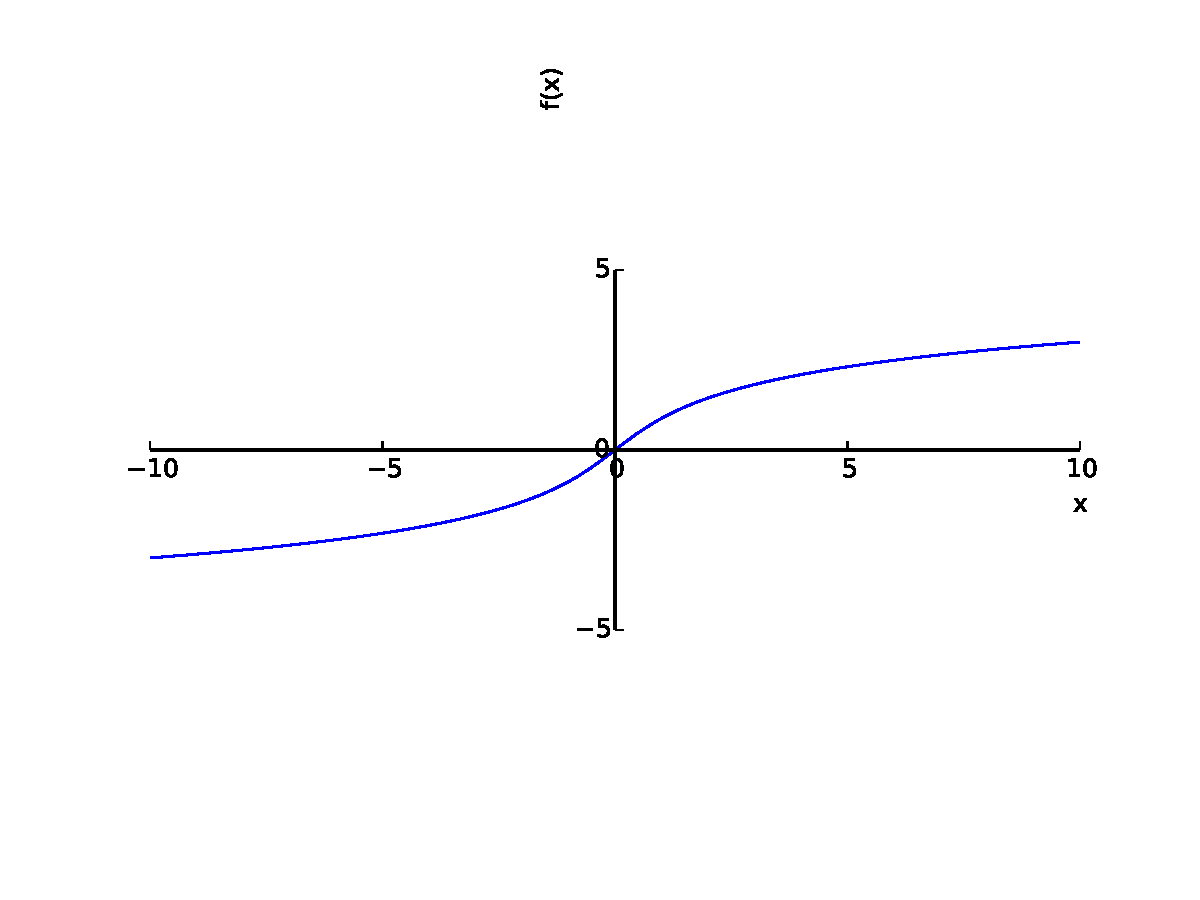
\includegraphics[width=0.8\textwidth]{beamer-pics/hyperbolics-4.pdf}
	\end{figure}

\end{frame}

\begin{frame}{Inverse Hyperbolic Functions}

	\begin{equation*}
		y = \cosh^{-1}(x)
	\end{equation*}

	\begin{figure}
		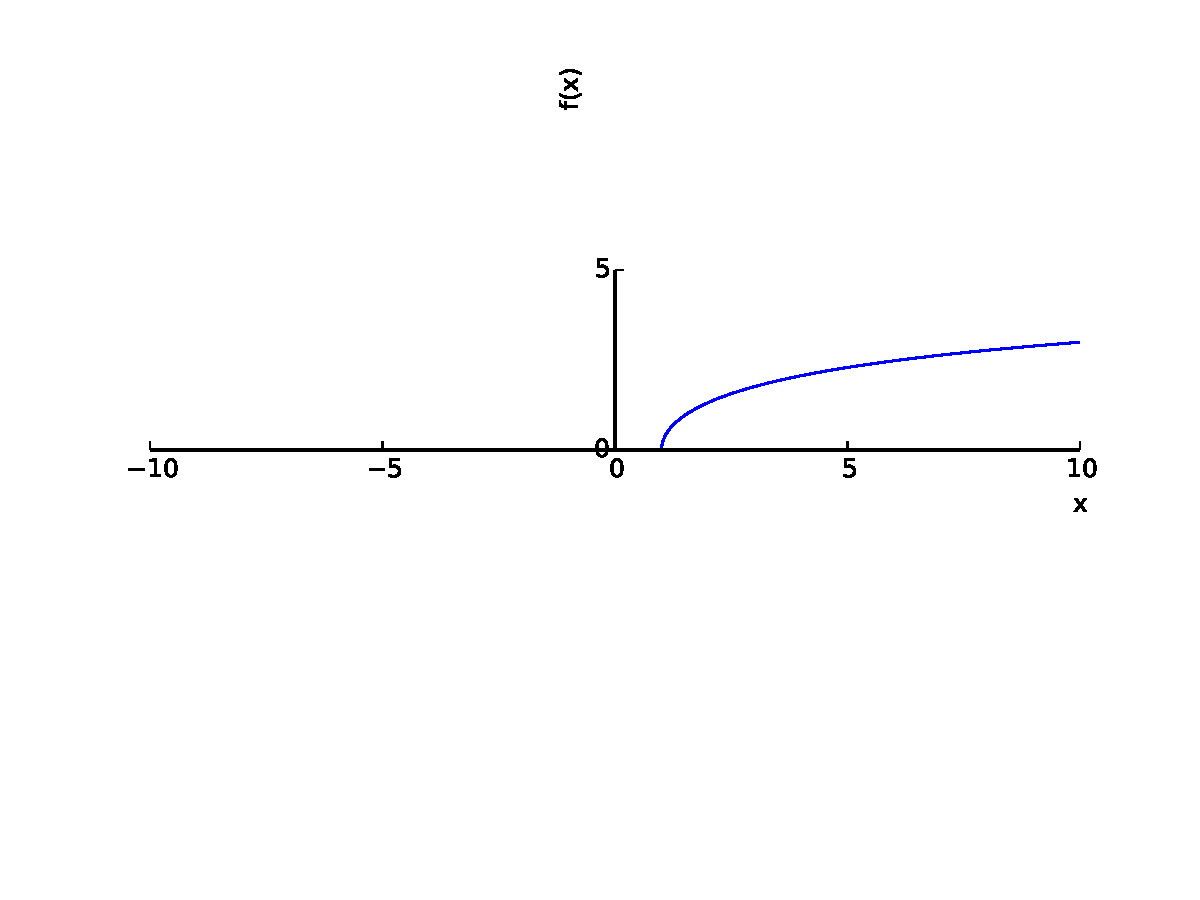
\includegraphics[width=0.9\textwidth]{beamer-pics/hyperbolics-5.pdf}
	\end{figure}

\end{frame}

\begin{frame}{Inverse Hyperbolic Functions}

	\begin{equation*}
		y = \tanh^{-1}(x)
	\end{equation*}

	\begin{figure}
		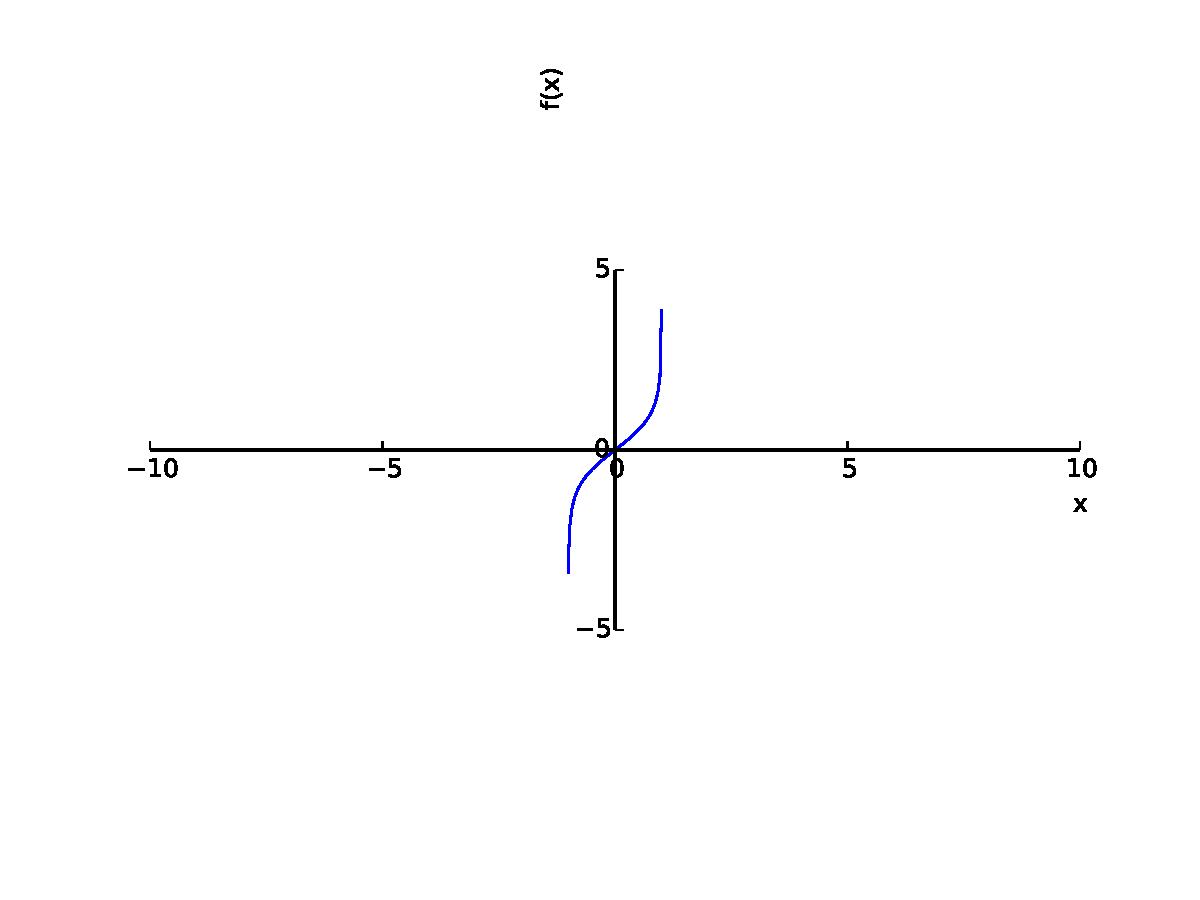
\includegraphics[width=0.9\textwidth]{beamer-pics/hyperbolics-6.pdf}
	\end{figure}

\end{frame}

\begin{frame}{Inverse Hyperbolic Functions}

	\textbf{Example:}
	
    Using implicit differentiation, find:
	
	\begin{align*}
		\frac{d}{dx}\left(\sinh^{-1}(x)\right) \only<2-> {&= \frac{1}{\sqrt{1+x^2}}}\\
		\frac{d}{dx}\left(\cosh^{-1}(x)\right) \only<3-> {&= \frac{1}{\sqrt{1-x^2}}}
	\end{align*}

\end{frame}

\begin{frame}{Standard Integrals}

	\begin{align*}
		\int\frac{1}{\sqrt{a^2-x^2}} &= \sin^{-1}\left(\frac{x}{a}\right) \hspace{3mm} (|x| < a) \\
		\int\frac{1}{a^2+x^2} &= \frac1a\tan^{-1}\left(\frac{x}{a}\right) \\
		\int\frac{1}{\sqrt{x^2-a^2}} &= \cosh^{-1}\left(\frac{x}{a}\right) = \ln\left(x + \sqrt{x^2 - a^2}\right) \hspace{3mm} (|x| < a) \\
		\int\frac{1}{\sqrt{x^2+a^2}} &= \sinh^{-1}\left(\frac{x}{a}\right) = \ln\left(x + \sqrt{x^2 + a^2}\right) \\
		\int\frac{1}{a^2-x^2} &= \frac1a\tanh^{-1}\left(\frac{x}{a}\right) = \frac{1}{2a}\ln\left|\frac{a+x}{a-x}\right| \hspace{2mm} (|x| < a) \\
		\int\frac{1}{x^2-a^2} &= \frac{1}{2a}\ln\left|\frac{x-a}{x+a}\right|
	\end{align*}

\end{frame}

\begin{frame}{Calculus with Hyperbolic Functions - Integration}

	\textbf{Examples:}
	
	Find the following:
	
	\begin{align*}
		\int \frac{1}{\sqrt{16+x^2}}dx \\
		\int \frac{1}{16+x^2}dx \\
		\int \frac{1}{x^2-25}dx \\
		\int \frac{1}{9-x^2}dx \\
		\int \frac{1}{\sqrt{9-x^2}}dx \\
		\int \frac{1}{\sqrt{x^2-25}}dx
	\end{align*}

\end{frame}

\end{document}
